\documentclass[twoside]{article}
\usepackage{amsgen,amsmath,amstext,amsbsy,amsopn,amssymb,color}
\usepackage{graphicx}
\usepackage{epsfig}

\setlength{\oddsidemargin}{0.1 in} \setlength{\evensidemargin}{-0.1
in} \setlength{\topmargin}{-0.6 in} \setlength{\textwidth}{6.5 in}
\setlength{\textheight}{10.5 in} \setlength{\headsep}{0.1 in}
\setlength{\parindent}{0 in} \setlength{\parskip}{0.1 in}

\newcommand{\red}{\textcolor{red}}

\newcommand{\homework}[2]{
   \pagestyle{myheadings}
   \thispagestyle{plain}
   \newpage
   \setcounter{page}{1}
   \noindent
   \begin{center}
   \framebox{
      \vbox{\vspace{2mm}
       \hbox to 6.28in { {\bf Math 4720:~Statistical Methods \hfill} }
       \vspace{6mm}
       \hbox to 6.28in { {\Large \hfill #1 (#2)  \hfill} }
       \vspace{6mm}
      \vspace{2mm}}
   }
   \end{center}
   \markboth{#1}{#1}
   \vspace*{4mm}
}

\newcommand{\bbF}{\mathbb{F}}
\newcommand{\bbX}{\mathbb{X}}
\newcommand{\bI}{\mathbf{I}}
\newcommand{\bX}{\mathbf{X}}
\newcommand{\bY}{\mathbf{Y}}
\newcommand{\bepsilon}{\boldsymbol{\epsilon}}
\newcommand{\balpha}{\boldsymbol{\alpha}}
\newcommand{\bbeta}{\boldsymbol{\beta}}
\newcommand{\0}{\mathbf{0}}

\begin{document}

\homework{$9^{th}$ Week Summary}{03/22/25}
\vspace{-0.4 in}
\begin{itemize}
\item \textbf{INFERENCE ABOUT POPULATION STANDARD DEVIATION}\dotfill
\item Test for the population standard deviation $(\sigma)$:
\subitem Given the data is coming from normal distribution we can use the chi-squared test to test 
\subitem $H_0: \sigma=\sigma_0$:
\subsubitem Test Statistics: $\chi^2=\dfrac{(n-1)s^2}{\sigma_0^2}$ follows $\chi^2(\nu=n-1)$
\subsubitem $100(1-\alpha)\%$ CI for $\sigma$: $\sqrt{\dfrac{(n-1)s^2}{\chi^2_{\alpha/2}}} < \sigma < \sqrt{\dfrac{(n-1)s^2}{\chi^2_{1-\alpha/2}}}$
\subsubitem R: \textsf{EnvStats::varTest(data, sigma.squared = 1)}
\item Test for the equality of the standard deviations $(H_0: \sigma_1 = \sigma_2)$:
\subitem Given the data-sets are coming from normal distribution we can use the F test to test
\subitem $H_0: \sigma_1=\sigma_2$
\subsubitem Test Statistics: $F=\dfrac{\max(s_1^2,s_2^2)}{\min(s_1^2,s_2^2)}$ follows $F(\nu_1=n_{num}-1,\nu_2=n_{den}-1)$
\subsubitem R: \textsf{var.test(x, y, ratio = 1)}
\item Test for  equality of the standard deviations for more than two populations $(H_0: \sigma_1=\sigma_2=\cdots=\sigma_t)$:
\subitem F test can be extended to more than two populations (Hartley's $F_{\max}$ test), but it is very sensitive to departures from normality.
\subitem We prefer to use Brown-Forsythe-\red{Levene}(BF\red{L}) test:
\subsubitem R: \textsf{lawstat::levene.test(data, group)}
\end{itemize}
\vspace{-.25in}\hrulefill\vspace{-.15in}
\begin{itemize}
\item \textbf{ANOVA}\dotfill
\item {ANalysis Of VAriance (ANOVA)} is a popular statistical tool to analyze the effect of a categorical variable with different levels of treatments (factor) on a numerical variable (response). 
\item In general, we can write:
$$\text{Total Variation} \;=\; \text{Variation Between Treatments} \;+\; \text{Variation Within Treatments}.$$
\vspace{-.25in}
\begin{figure}[h]
\begin{center}
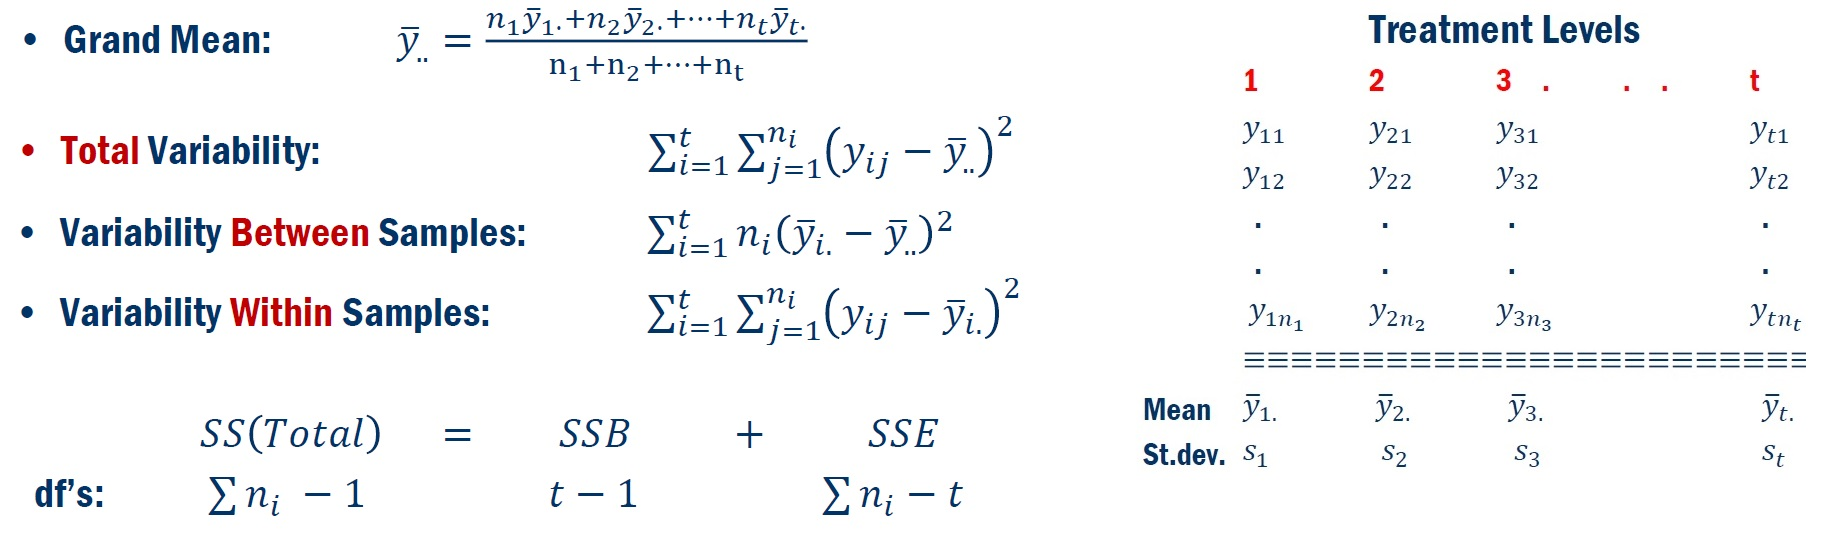
\includegraphics[angle=0, width=15 cm] {ANOVA_data.jpg}
\end{center}
\end{figure}
\vspace{-.25in}
\item Hypothesis Testing
\subitem $H_0: \mu_1 = \mu_2 = \cdots = \mu_t$
\subitem $H_a: \mu_i \neq \mu_j \;\; \text{for some pair } (i, j).$
\subitem Test Statistic: $F = \dfrac{{SSB}/{{df}_B}}{{SSE}/{{df}_E}}$
\subitem Decision Rule: Reject $H_0$ in favor of $H_a$ if $F > F_{\alpha}({df}_B, {df}_E)$.
\end{itemize}

\end{document}


